%%%%%%%%%%%%%%%%%%%%%%%%%%%%%%%%%%%%%%%%%%%%%%%%%
% Laatste aanpassing:
% 6 sept 2013 [Jan]: kleine foutjes en lay-out verbeterd
%                           
% 11/9/2012 [Greetje] aangepast aan hoofdstuk eerstegraadsfuncties
% mei 2011 [Jan]: Figuren in TikZ, tabellen in booktabs, enkele foutjes verbeterd, voor eenheden siunitx gebruikt, getallen met decimale punt in \num 
%
% 23/03/11 [Greetje]: Volledige herwerking
%
% 19/9/02 [Jan]: figuur van lin. en exp. groei opnieuw
%	gemaakt (fig_ weggedaan in de naam van het bestand).
%                   
% 9/9/02 [Jan]: figuren in aparte map. Verwijzingen naar Mathcad
%    weggewerkt.
%                                               
% 04/08/02 door Roby                            
%   tekeningen aangepast aan Euler 
%             
% 10/09/01 door Greetje                         
%   typfouten van Roby vervangen                
%   $m$ uniform vervangen door \SI{•}{•}m                
%   \vspace{0.3cm} tussen caption en tabel 
%     
% 01/09/01 door Greetje                         
%%%%%%%%%%%%%%%%%%%%%%%%%%%%%%%%%%%%%%%%%%%%%%%%%



\chapter{Exponenti\"{e}le groeiprocessen}\label{chap:groei}
\begin{quote}
     \textit{{\small `Vreemderder en vreemderder!' riep Alice. (Ze was zo stomverbaasd
              dat ze eventjes compleet vergeten was hoe je ook alweer goed
              Nederlands sprak.) `Nu schuif ik uit als de grootste telescoop die
              er ooit geweest is! Vaarwel voeten!' (Want toen ze neerkeek op haar
              voeten waren ze bijna uit zicht, leek het wel, zo ver raakten ze
              weg.) `Ach, mijn arme voetjes, ik vraag me af wie jullie nu moet
              helpen bij het aantrekken van schoenen en kousen, schatten van me.
              \emph{Ik} kan het vast niet meer! Ik sta er veel te ver van af om
              me nog druk te maken over jullie. Maak er het beste van' -- maar
              ik moet aardig tegen ze zijn, dacht Alice, anders lopen ze niet
              de kant op die ik wil! Eens even denken: voortaan krijgen ze met
              de kerst nieuwe laarzen van me.}}

          Uit `Alice in Wonderland' -- Lewis Carroll
\end{quote}

\newpage
\section{Groeiprocessen: een voorbeeld}
In deze sectie behandelen we enkele modellen van groei. Het eenvoudigste model, dat in de natuur zelden voorkomt, is dat van lineaire groei. Hierbij is de aangroei per tijdseenheid constant. Meer re\"eel is het exponentieel groeimodel, waarbij de procentuele aangroei constant is. We beginnen met een voorbeeld.

\label{page:meeralgen}
\begin{quote}
    Een meer is nu \SI{800}{\square\meter} groot. Elke week wordt er \SI{550}{\square\meter} uitgegraven, zodat de oppervlakte van het meer steeds
toeneemt. Men wil het meer voor recreatie gebruiken, maar nu zijn
er reeds \SI{5}{\square\meter} algen aan de oppervlakte aanwezig. Men schat
dat de oppervlakte algen per week verdubbelt. De uitbater vindt
dat er dringend moet ingegrepen worden, maar de burgemeester ziet
geen probleem aangezien het meer ook elke week groter wordt.
Zal er steeds een gedeelte van het meer algenvrij blijven of niet?
\end{quote}
Dit voorbeeld bevat twee verschillende groeiprocessen: de aangroei van de
oppervlakte van het meer en de aangroei van de oppervlakte bedekt met algen.
We gaan na op welke manier beide processen van mekaar verschillen.

\subsection{Lineaire groei}
We bekijken eerst de groei van de oppervlakte van het meer. Zoals we gedaan hebben in hoofdstuk~\ref{chap:eerstegraadsfuncties} stellen we eerst het wiskundig model op. 
De oppervlakte benoemen we met de functie $M(t)$, met $t$ de veranderlijke tijd, uitgedrukt in weken.
Van deze functie weten we het volgende:

\begin{itemize}
  \item  Als $t=0$ dan is $M(0)=800$
  \item  Als $t=1$ dan is $M(1)=800+1\cdot 550=1350$
  \item  Als $t=3$ dan is $M(3)=800+3\cdot 550=2450$
  \item  \ldots
\end{itemize}

Dit wordt weergegeven in tabel~\ref{tabel:meer} (vergelijk met tabel~\ref{tbl:taxi} op pagina~\pageref{tbl:taxi}).
 \begin{table}[htb]
    \centering
    \vspace{0.3cm}
        \caption{De groei van de oppervlakte  van het meer.}
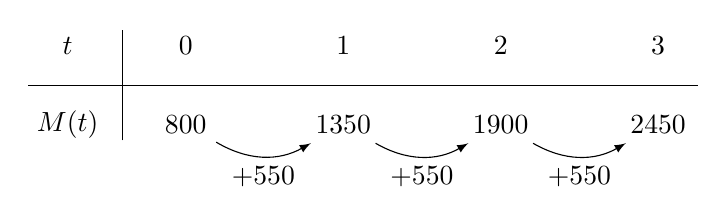
\begin{tikzpicture}
\node at (1.5,3) {$t$};
\node at (3,3)  {0};
\node at (5,3)  {1};
\node at (7,3)  {2};
\node at (9,3)  {3};
\node at (1.5,2)  {$M(t)$};
\node (M1) at (3,2)  {800};
\node (M2) at (5,2)  {1350};
\node (M3) at (7,2)  {1900};
\node (M4) at (9,2)  {2450};
\draw (1,2.5) -- (9.5,2.5);
\draw (2.2,1.8) -- (2.2,3.2	);
\draw[-latex] (M1) to [bend right]  node [below] {$+550$} (M2);
\draw[-latex] (M2) to [bend right]  node [below] {$+550$} (M3);
\draw[-latex] (M3) to [bend right]  node [below] {$+550$} (M4);
\end{tikzpicture}
\label{tabel:meer}
 \end{table}
 
\noindent
Hieruit leiden we  het voorschrift voor de functie $M(t)$ af.
\begin{displaymath}
    M(t)=800+t\cdot 550
\end{displaymath}
Dit is de vergelijking van  een eerstegraads- of lineaire functie. Elke week wordt  eenzelfde hoeveelheid oppervlakte \emph{opgeteld}. We spreken van \emph{lineaire groei}\index{lineaire groei}. We nemen aan dat de graafmachines de hele dag doorwerken (ook 's nachts). De veranderlijke $t$ hoeft dus geen geheel getal te zijn, maar kan een willekeurig positief reëel getal zijn. Het domein van de functie $M(t)$ is dus $\real^+$. 


Het volgend verband is onmiddellijk duidelijk:
\begin{displaymath}
    M(t)=M(t-1) +550
\end{displaymath}
 Dit verband noemen we \emph{recursief}\index{recursief}, omdat de hoeveelheid van deze  week $M(t)$ uitgedrukt wordt in functie van de hoeveelheid van de vorige week $M(t-1)$.

De grafiek van de functie $M(t)$ is een rechte (zie figuur~\ref{fig:lingroei}). Het getal $550$ is de richtingsco\"effici\"ent van de rechte. De grafiek snijdt de verticale as in $800$ (de beginwaarde $M(0)$ van het groeiproces).   Deze grafiek is typisch voor elk lineair groeiproces (vergelijk met sectie~\ref{subsec:grafischeVoorstelling}).
\begin{figure}[tbp]
    \centering
\begin{tikzpicture}[line cap=round,line join=round,x=1.0cm,y=0.0015cm]
\draw[->] (0,0) -- (5,0) node [at end, below] {$t$};
\foreach \x in {1,2,3,4}
\draw[shift={(\x,0)}] (0pt,2pt) -- (0pt,-2pt) node[below] {\footnotesize $\x$};
\draw[->] (0,0) -- (0,3500) node [at end, left] {$M(t)$};
\foreach \y in {1000,2000,3000}
\draw[shift={(0,\y)},color=black] (2pt,0pt) -- (-2pt,0pt) node[left] {\footnotesize $\y$};
\draw[color=black] (0pt,-10pt) node[right] {\footnotesize $0$};
%\clip(-0.52,0) rectangle (5.1,3900);
\draw [domain=-0:4,thick] plot(\x,{(--800--550*\x)/1});
\draw [dashed, gray] (2,0) |- (0,1900);
\draw [dashed, gray] (3,0) |- (0,2450);
\draw[-latex,red] (2,1900) to node[below] {$+1$} (3,1900) ;
\draw[-latex,red] (3,1900) to node[right] {$+550$} (3,2450) ;
\end{tikzpicture}
    \caption{Aangroei van de oppervlakte van het meer $M(t)=800+t\cdot 550$}
    \label{fig:lingroei}
\end{figure}

\subsection{Exponenti\"{e}le groei.}
\label{subsec: exp_groei_vb}
We herhalen hetzelfde voor de groei van de algen. We
noemen de groeifunctie $A(t)$,
met $t$ de tijd uitgedrukt in weken.
Van deze functie weten we het volgende:
\begin{itemize}
    \item  Als $t=0$ dan is $A(0)=5$

    \item  Als $t=1$ dan is $A(1)=5\cdot 2=10$

    \item  Als $t=2$ dan is $A(2)=A(1)\cdot 2=(5\cdot 2)\cdot 2=5\cdot 2^{2}$

    \item  Als $t=3$ dan is $A(3)=A(2)\cdot 2=(5\cdot 2^{2})\cdot 2=5\cdot 2^{3}$

    \item  \ldots
\end{itemize}
Als we kijken waar we de waarde van $t$ terugvinden in de
rechteruitdrukkingen, dan vinden we als voorschrift
\begin{equation}
    A(t)=5\cdot 2^{t}
    \label{eq:algen}
\end{equation}


 \begin{table}[htb]
    \centering
        \caption{De groei van de algen  van het meer.}
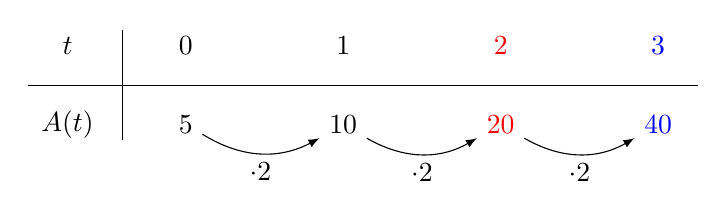
\begin{tikzpicture}
\node at (1.5,3) {$t$};
\node at (3,3)  {0};
\node at (5,3)  {1};
\node at (7,3) [red]  {2};
\node at (9,3) [blue] {3};
\node at (1.5,2)  {$A(t)$};
\node (M1) at (3,2)  {5};
\node (M2) at (5,2)  {10};
\node (M3) at (7,2) [red] {20};
\node (M4) at (9,2) [blue]  {40};
\draw (1,2.5) -- (9.5,2.5);
\draw (2.2,1.8) -- (2.2,3.2	);
\draw[-latex] (M1) to [bend right]  node [below] {$\cdot 2$} (M2);
\draw[-latex] (M2) to [bend right]  node [below] {$\cdot 2$} (M3);
\draw[-latex] (M3) to [bend right]  node [below] {$\cdot 2$} (M4);
\end{tikzpicture}
\label{tabel:algen}
 \end{table}
In tabel~\ref{tabel:algen} geven we de groei schematisch weer. 

We spreken van \emph{exponenti\"ele groei}\index{exponenti\"ele groei} omdat de oppervlakte bedekt met algen elke week
\emph{vermenigvuldigd} wordt met eenzelfde factor, hier $2$. We noemen dit getal de \emph{groeifactor}. Het getal 5 geeft aan hoeveel algen er zijn op begintijdstip $t=0$. We noemen 5 dan ook de \emph{beginwaarde}.

De groei van de algen gebeurt continu:  na een halve week is de hoeveelheid reeds toegenomen. Als we er vanuit gaan dat de groeifactor de eerste helft van de week dezelfde is als de tweede helft van de week (zie figuur~\ref{fig:algen_periode2}), dan blijkt dat de veranderlijke $t$ in vergelijking~\eqref{eq:algen} geen geheel getal hoeft te zijn. Het domein van de functie $A(t)$ is dus $\real^+$.

\begin{figure}[htbp]
    \centering
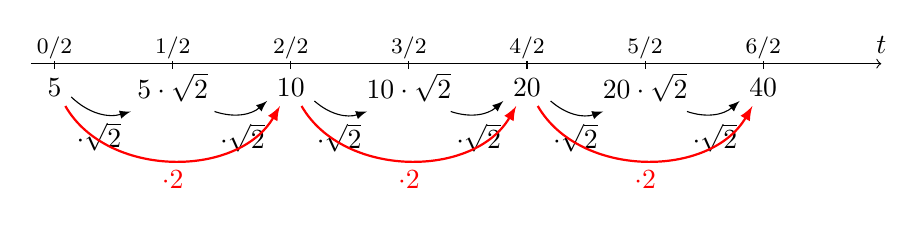
\begin{tikzpicture}[x=1.5cm]
\draw[->] (-0.2,0.3) -- (7,0.3) node [at end, above] {$t$};
\foreach \x in {0,...,6}
\draw[shift={(\x,0.3)}] (0pt,1pt) -- (0pt,-2pt) node[above] {\footnotesize $\x/2$};
\node (M1) at (0,0) {5};
\node (M2) at (1,0) {$5\cdot\sqrt{2}$};
\node (M3) at (2,0) {10};
\node (M4) at (3,0) {$10\cdot\sqrt{2}$};
\node (M5) at (4,0) {20};
\node (M6) at (5,0) {$20\cdot\sqrt{2}$};
\node (M7) at (6,0) {40};
\draw[-latex] (M1) to [bend right]  node [below] {$\cdot \sqrt{2}$} (M2);
\draw[-latex] (M2) to [bend right]  node [below] {$\cdot \sqrt{2}$} (M3);
\draw[-latex,color=red,thick] (M1) to [out=-60,in=-120]  node [below] {$\cdot 2$} (M3);
\draw[-latex] (M3) to [bend right]  node [below] {$\cdot \sqrt{2}$} (M4);
\draw[-latex] (M4) to [bend right]  node [below] {$\cdot \sqrt{2}$} (M5);
\draw[-latex,color=red,thick] (M3) to [out=-60,in=-120]  node [below] {$\cdot 2$} (M5);
\draw[-latex] (M5) to [bend right]  node [below] {$\cdot \sqrt{2}$} (M6);
\draw[-latex] (M6) to [bend right]  node [below] {$\cdot \sqrt{2}$} (M7);
\draw[-latex,color=red,thick] (M5) to [out=-60,in=-120]  node [below] {$\cdot 2$} (M7);
\end{tikzpicture}
    \caption{Groeifactor van de aangroei van de algen verandert als de periode verandert }
    \label{fig:algen_periode2}
\end{figure}

Het volgend verband is voor iedereen onmiddellijk duidelijk:
\[A(t)=A(t-1)\cdot 2
\] 
Dit is opnieuw een \emph{recursief}\index{recursief} voorschrift.

Zoals je ziet op figuur~\ref{fig:algen}, is de grafiek van $A(t)$ geen rechte meer. Omdat de veranderlijke $t$
in vergelijking~\eqref{eq:algen} in de exponent staat noemen we $A(t)$  een \emph{exponenti\"{e}le
functie}. De groeifactor $2$ is het grondtal\index{grondtal} van de exponenti\"ele functie.
De beginwaarde $5$ is het snijpunt van de functie met de verticale as. In hoofdstuk~\ref{chap:expFunctie} gaan we dieper in op exponentiële functies.
\begin{figure}[tbp]
    \centering
    \begin{tikzpicture}[line cap=round,line join=round,x=1.0cm,y=0.05cm]
    \draw[->] (-2.2,0) -- (5.5,0) node [at end, below] {$t$};
    \foreach \x in {-1,0,1,2,3,4,5}
    \draw[shift={(\x,0)}] (0pt,2pt) -- (0pt,-2pt) node[below] {\footnotesize $\x$};
    \draw[->] (0,0) -- (0,170) node [at end, left] {$A(t)$};
    \foreach \y in {20,40,...,160}
    \draw[shift={(0,\y)},color=black] (2pt,0pt) -- (-2pt,0pt) node[left] {\footnotesize $\y$};
    \draw [domain=-2:5,thick] plot(\x,{5*exp(\x*ln(2))});
    \draw [dashed, gray] (2,0) |- (0,20);
    \draw [dashed, gray] (3,0) |- (0,40);
        \filldraw [red] (2,20) circle (2pt);
            \filldraw [blue] (3,40) circle (2pt);
    \end{tikzpicture}
    \caption{Aangroei van de oppervlakte bedekt met algen $A(t)=5\cdot 2^{t}$}
    \label{fig:algen}
\end{figure}


\subsection{Vergelijking van de twee groeiprocessen.}
\begin{figure}[tbp]
    \centering
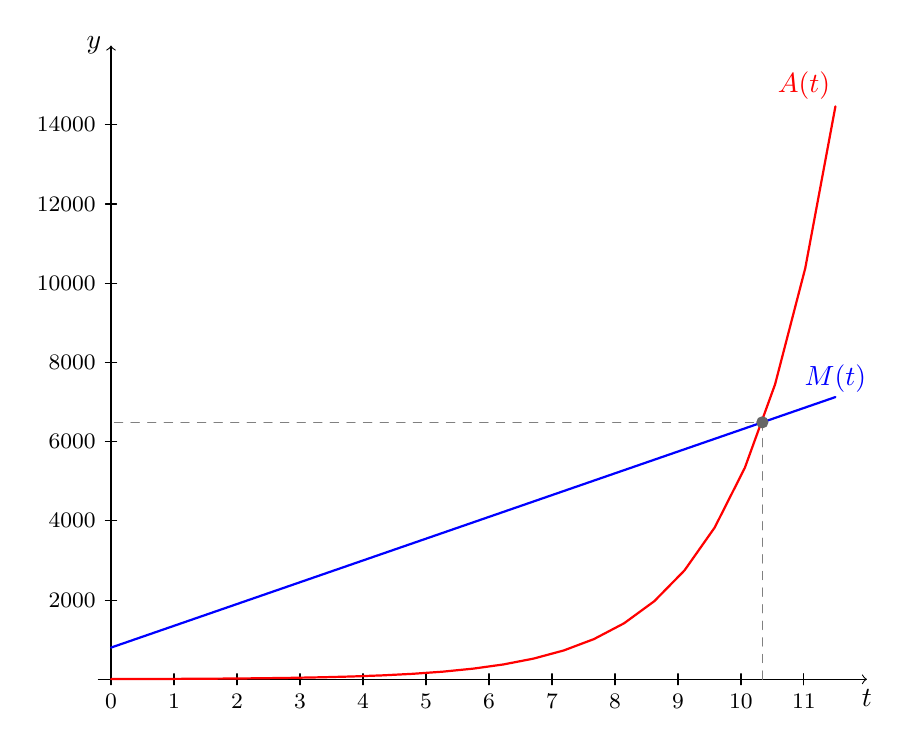
\begin{tikzpicture}[line cap=round,line join=round,x=0.8cm,y=0.0005cm]
\draw[->] (-0.2,0) -- (12,0) node [at end, below] {$t$};
\foreach \x in {0,...,11}
\draw[shift={(\x,0)}] (0pt,2pt) -- (0pt,-2pt) node[below] {\footnotesize $\x$};
\draw[->] (0,0) -- (0,16000) node [at end, left] {$y$};
\foreach \y in {2000,4000,6000,8000,10000,12000,14000}
\draw[shift={(0,\y)},color=black] (2pt,0pt) -- (-2pt,0pt) node[left] {\footnotesize $\y$};
\draw [domain=0:11.5,thick,color=red] plot(\x,{5*exp(\x*ln(2))});
\draw [domain=-0:11.5,thick,color=blue] plot(\x,{(--800--550*\x)/1});
\draw [dashed, gray] (10.34,0) |- (0,6488);
\node at (11,15000) [red] {$A(t)$};
\node at (11.5,7600) [blue] {$M(t)$};
    \filldraw [black!60] (10.34,6488) circle (2pt);
\end{tikzpicture}
    \caption{Aangroei van de oppervlakte van het meer $M(t)=800+t\cdot 550$ en aangroei van de oppervlakte bedekt met algen $A(t)=5\cdot 2^{t}$}
    \label{fig:linexp}
\end{figure}

In figuur~\ref{fig:linexp} vind je de grafieken van $A(t)$ en
$M(t)$ op \'{e}\'{e}n tekening. We zien duidelijk
dat de groei van de oppervlakte bedekt met algen
in het begin traag gaat, want er zijn weinig algen. Zodra
er meer algen zijn, groeien die veel sneller aan en zullen ze
het ganse meer overwoekeren. Op de grafiek lezen we af dat
tussen de $10$ en de $11$ weken het meer overwoekerd is door algen.
Dezelfde oplossing lezen we af op
tabel~\ref{tbl:meeralgen}, waar de resultaten per week van beide
groeiprocessen weergegeven worden.
\begin{table}[htb]
    \centering
    \caption{De groei van de algen en de oppervlakte van het meer.}
    \begin{tabular}{rrcr}
    \toprule
    $t$ & $A(t)$ & verband & $M(t)$  \\
    \midrule
    0 & 5 & ${\color{red}<}$ & 800  \\
    1 & 10 & ${\color{red}<}$ & 1350  \\
    2 & 20 & ${\color{red}<}$ & 1900  \\
    3 & 40 &  ${\color{red}<}$ & 2450  \\
    4 & 80 &  ${\color{red}<}$ & 3000  \\
    5 & 160 &  ${\color{red}<}$ & 3550  \\
    6 & 320 &  ${\color{red}<}$ & 4100  \\
    7 & 640 &  ${\color{red}<}$ & 4650  \\
    8 & 1280 &  ${\color{red}<}$ & 5200  \\
    9 & 2560 & ${\color{red}<}$ & 5750  \\
    10 & 5120 &  ${\color{red}<}$ & 6300  \\
    \cmidrule{2-4}
    11 & 10240 & ${\color{blue}>}$ & 6850  \\
    12 & 20480 & ${\color{blue}>}$ & 7400 \\
    \bottomrule
\end{tabular}
    \label{tbl:meeralgen}
\end{table}

We kunnen het moment dat het meer vol algen zit ook berekenen met formules. De uitgegraven oppervlakte is gelijk aan de oppervlakte bedekt met algen als
\begin{displaymath}
    800+550\cdot t=5\cdot 2^{t}
\end{displaymath}
Deze vergelijking ziet er vrij eenvoudig uit. Nochtans kan ze niet
opgelost worden met de methoden van sectie~\ref{sec:exp_vgl}.  We kunnen ze alleen
 benaderend oplossen met de computer. Als we een algoritme zouden programmeren en dit toepassen, vinden we $t=\num{10.342}$ weken. \\
 
 \noindent
\textbf {Besluit:} Wil de burgemeester dit gebied als recreatiezone gebruiken
 dan moet hij de groei van de algen drastisch indijken.



\newpage
\section{Exponenti\"ele groei}
\subsection{Definities}

We veralgemenen vergelijking (\ref{eq:algen}) van sectie~\ref{subsec: exp_groei_vb}. 
\begin{quote}

Zij  $B(t)$ de functie die de exponenti\"{e}le
aangroei van een grootheid weergeeft, waarbij $t$ uitgedrukt is in aantal \emph{perioden}\index{periode} (bijvoorbeeld weken, uren, meter, centimeter). De \emph{groeifactor}\index{groeifactor} $g$ is de factor waarmee de functie per periode toeneemt (vermenigvuldigd wordt). Bij het begin van de meting ($t=0$) heeft de functie \emph{beginwaarde}\index{beginwaarde} $B(0)$. Dan is het functievoorschrift van deze functie
\begin{equation}
    B(t)=B(0)\cdot g^{t}
    \label{eq:eq_groei2}
\end{equation}
Het domein van de functie $B(t)$ is $\real^+$.

\end{quote}
De recursieve formule is :
\begin{equation}
    B(t)=B(t-1)\cdot g
\end{equation}
want $g$ is \emph{onafhankelijk} van het moment waarop men de periode laat
beginnen.



De groeifactor is \emph{wel} afhankelijk van de
lengte van de periode. We nemen terug het voorbeeld van sectie~\ref{subsec: exp_groei_vb}.  In het voorbeeld wordt de aangroei \emph{per week}  bekeken: week na week moet je de hoeveelheid algen vermenigvuldigen met twee (periode: 1 week; groeifactor: 2). Wat als je de aangroei van de algen per 3 weken wil meten (periode: 3 weken)? In figuur~\ref{fig:algen_periode} zie je dat in dat geval de hoeveelheid algen per periode drie keer na mekaar met 2 vermenigvuldigd moet worden, dus met $2^3=8$. Als de periode 3 weken bedraagt, is de groeifactor gelijk aan 8.
\begin{figure}[htbp]
    \centering
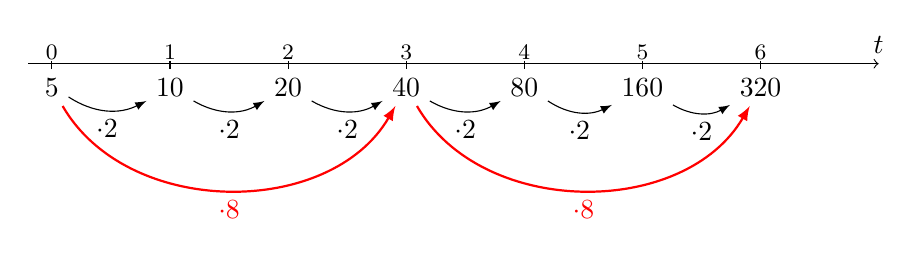
\begin{tikzpicture}[x=1.5cm]
\draw[->] (-0.2,0.3) -- (7,0.3) node [at end, above] {$t$};
\foreach \x in {0,...,6}
\draw[shift={(\x,0.3)}] (0pt,1pt) -- (0pt,-2pt) node[above] {\footnotesize $\x$};
\node (M1) at (0,0) {5};
\node (M2) at (1,0) {10};
\node (M3) at (2,0) {20};
\node (M4) at (3,0) {40};
\node (M5) at (4,0) {80};
\node (M6) at (5,0) {160};
\node (M7) at (6,0) {320};
\draw[-latex] (M1) to [bend right]  node [below] {$\cdot 2$} (M2);
\draw[-latex] (M2) to [bend right]  node [below] {$\cdot 2$} (M3);
\draw[-latex] (M3) to [bend right]  node [below] {$\cdot 2$} (M4);
\draw[-latex,color=red,thick] (M1) to [out=-60,in=-120]  node [below] {$\cdot 8$} (M4);
\draw[-latex] (M4) to [bend right]  node [below] {$\cdot 2$} (M5);
\draw[-latex] (M5) to [bend right]  node [below] {$\cdot 2$} (M6);
\draw[-latex] (M6) to [bend right]  node [below] {$\cdot 2$} (M7);
\draw[-latex,color=red,thick] (M4) to [out=-60,in=-120]  node [below] {$\cdot 8$} (M7);
\end{tikzpicture}
    \caption{Groeifactor van de aangroei van de algen verandert als de periode verandert }
    \label{fig:algen_periode}
\end{figure}

In het algemeen komt het op het volgende neer: als je de periode vermenigvuldigt met een factor $k$, moet je de groeifactor tot de $k$-de macht verheffen. Dit wordt schematisch weergegeven in figuur~\ref{fig:periode_factor}.
\begin{figure}[tbp]
    \centering
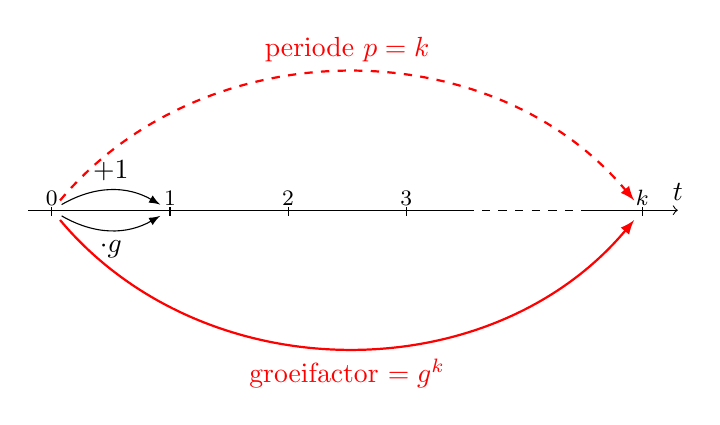
\begin{tikzpicture}[x=1.5cm]
\draw[dashed](3.5,0.0)--(4.5,0.0);
\draw[] (-0.2,0.0) -- (3.5,0.0);
\draw[->] (4.5,0.0) -- (5.3,0.0) node [at end, above] {$t$};
\foreach \x in {0,1,2,3}
\draw[shift={(\x,0.0)}] (0pt,1pt) -- (0pt,-2pt) node[above] {\footnotesize $\x$};
\draw[shift={(5,0.0)}] (0pt,1pt) -- (0pt,-2pt) node[above] {\footnotesize $k$};
\node (M1) at (0,0) {};
\node (M2) at (1,0) {};
\node (M3) at (2,0) {};
\node (M4) at (3,0) {};
\node (Mk) at (5,0) {};
\draw[-latex] (M1) to [bend right]  node [below] {$\cdot g$} (M2);
\draw[-latex] (M1) to [bend left]  node [above] {$+1$} (M2);
\draw[-latex,color=red,thick] (M1) to [out=-50,in=-130]  node [below] {groeifactor $= g^k$} (Mk);
\draw[-latex,color=red,thick,dashed] (M1) to [out=50,in=130]  node [above] {periode $p=k$} (Mk);
\end{tikzpicture}
    \caption{Relatie tussen periode $p$ en groeifactor}
    \label{fig:periode_factor}
\end{figure}
Als de periode kleiner wordt, is de factor $k$ kleiner dan 1. Als in het algenprobleem de periode gelijk is aan 1 dag (=1/7 van een week), is de groeifactor $2^{1/7}$.

In elk probleem is de
keuze van de periode vrij te kiezen, maar de groeifactor zal door die
keuze bepaald worden.\\


We besluiten: een exponentieel groeiproces wordt gekenmerkt door drie elementen:
\begin{enumerate}
\item de beginwaarde $K(0)$
\item de periode $p$
\item de groeifactor $g$
\end{enumerate}
Het functievoorschrift van het groeiproces is dan 
\begin{equation}
K(t)=K(0)\cdot g^t
\label{eq:exp_groei}
\end{equation}
Het domein van het groeiproces is $\real^+$.
Merk op dat de veranderlijke $t$ niet steeds een tijd is. De veranderlijke kan ook een afstand zijn, de diepte, de hoogte \dots.

Vaak worden opeenvolgende metingen van een experiment gebruikt om de toestand van de opstelling te achterhalen  \emph{voor} het begin van de meting. Als het zinvol is, kan de veranderlijke $t$ dan een negatieve waarde aannemen. 

\subsection{Stijgend groeiproces}\label{subsec:stijgendGroeiproces}
In het voorbeeld van sectie~\ref{subsec: exp_groei_vb} neemt de grootheid $A(t)$ toe in de tijd: de
oppervlakte bedekt met algen wordt steeds groter. We noemen dit dan
ook een stijgend groeiproces. In wat volgt geven we nog een voorbeeld van een stijgend
groeiproces. 

\subsubsection{Voorbeeld: samengestelde intrest}\label{subsubsec.si}
Als je geld stort op je spaarboekje, krijg je vanaf de eerste dag reeds intrest. Deze intrest wordt bij het kapitaal geteld en brengt op zijn beurt opnieuw intrest op. Dit noemen we samengestelde intrest.
\begin{quote}
    Een kapitaal van \euros{1000} staat gedurende 10 jaar uit tegen een
jaarlijkse rentevoet van \SI{7}{\percent}. Hoe groot is dit kapitaal na 10
jaar?
\end{quote}
Is het hierboven beschreven proces inderdaad een exponentieel groeiproces? 
We noemen de functie die het kapitaal
weergeeft in functie van de tijd $K(t)$, met $t$ uitgedrukt in jaren.
In tabel~\ref{tbl:groeikap} berekenen we het kapitaal voor drie opeenvolgende jaren.
\begin{table}[tbp]
    \centering
    \caption{De groei van het kapitaal per jaar}
    \begin{tabular}{ll}
    \toprule
    $t$ & $K(t)$\\
    \midrule
    $0$ 	& $K(0)=1000$ 	\\
    $1$	&$K(1)=K(0)+K(0)\cdot \num{0.07}=  K(0)\cdot \num{1.07}=1070$\\
   $2$	&$K(2)=K(1)+K(1)\cdot \num{0.07}= K(1)\cdot \num{1.07}=\num{1144.9}$ \\
   $3$	&$K(3)=K(2)+K(2)\cdot \num{0.07}= K(2)\cdot \num{1.07}=\num{1225.043}$ \\
\bottomrule
\end{tabular}
\label{tbl:groeikap}
\end{table}
Als we in deze tabel alle getallen samenvatten op een tijdsas bekomen we figuur~\ref{fig:kapitaalgroei}.
\begin{figure}[htbp]
    \centering
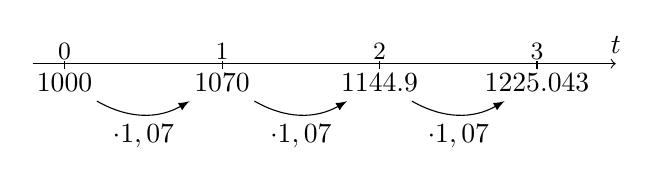
\begin{tikzpicture}[x=2cm]
\draw[->] (-0.2,0) -- (3.5,0) node [at end, above] {$t$};
\foreach \x/\y in {0/1000,1/1070,2/\num{1144.9},3/\num{1225.043}}{
	\draw[shift={(\x,0.0)}] (0pt,1pt) -- (0pt,-2pt) node[above] {\small $\x$};
	\node (\x) [below] at (\x,0) {\y};
}
\foreach \x/\y in {0/1,1/2,2/3}
	\draw[-latex] (\x) to [bend right]  node [below] {$\cdot 1,07$} (\y);
\end{tikzpicture}
    \caption{Groei van kapitaal van \euros{1000} tegen een WR van \SI{7}{\percent}}
    \label{fig:kapitaalgroei} 
\end{figure}



We merken het volgende:
\begin{enumerate}
\item De beginwaarde is gelijk aan $K(0)=1000$.
\item Uit de opgave blijkt dat de periode gelijk is aan 1 jaar.
\item Jaar na jaar wordt het kapitaal vermenigvuldigd met $\num{1.07}$. De groeifactor $g$ is dus gelijk aan \num{1.07}.
\end{enumerate}
Het hierboven beschreven proces is inderdaad een exponentieel groeiproces. Uit vergelijking~(\ref{eq:exp_groei}) volgt dat het voorschrift gegeven is door 
\begin{equation}
     K(t)=K(0)\cdot g^{t}=1000\cdot \num{1.07}^{t}
    \label{eq:si}
\end{equation}

Om het kapitaal na 10 jaar te berekenen, hoeven we enkel $K(10)=1000\cdot \num{1.07}^{10}=1967,15$ te berekenen. We vinden een kapitaal van \euros{1967,15}.

\subsubsection{Procentuele toename}
Hoe verandert de absolute toename $V(t)=K(t)-K(t-1)$ per periode (tijdseenheid) in een
exponentieel groeiproces?  We berekenen enkele van die toenamen in
tabel~\ref{tbl:samgesint} (derde kolom). 
\begin{table}[htb]
    \centering
    \caption{De \emph{toename} van het kapitaal per jaar}
    \begin{tabular}{cccc}
     \toprule
    $t$ & $K(t)$ & $V(t)=K(t)-K(t-1)$  & $ P(t)=\dfrac{V(t)}{K(t-1)}$\\
    \midrule
    0 & 1000 &   &\\

    1 & 1070 & 70&$\dfrac{70}{1000}=\num{0.07}$   \\[10pt]

    2 & \num{1144,9} & \num{74,9} & $\dfrac{\num{74.9}}{1070}=\num{0.07}$  \\[10pt]

    3 & \num{1225,043} & \num{80,14} &$\dfrac{\num{80.14}}{\num{1144.9}}=\num{0.07}$ \\[10pt]

    4 & \num{1310,796} & \num{85,75}  & $\dfrac{\num{85,75}}{\num{1225,043}}=\num{0.07}$\\
    \bottomrule
\end{tabular}
    \label{tbl:samgesint}
\end{table}

Uit tabel~\ref{tbl:samgesint}  blijkt dat de absolute toename jaar na jaar toeneemt. Dit is typisch voor een exponentieel groeiproces. 
 Bij lineaire groei is deze absolute toename constant. Daardoor is de grafiek van een lineair groeiproces een rechte en die van een exponentieel groeiproces niet.
 
 Berekenen we echter de
 \emph{procentuele jaarlijkse toename} $P(t)$,  de verhouding van de
 absolute toename $V(t)$ tot het kapitaal dat er was bij het vorige tijdstip $K(t-1)$ (vierde kolom in tabel~\ref{tbl:samgesint})
 \begin{displaymath}
     P(t)=\frac{V(t)}{K(t-1)}
 \end{displaymath}
We zien dat de procentuele toename per periode wel
constant is. De procentuele toename blijkt gelijk te zijn aan de groeifactor $g=\num{1.07}$ verminderd met 1.

We besluiten: een groeiproces met procentuele toename van $p$\,\%
 per periode, heeft per
 tijdseenheid een groeifactor 
 \begin{equation}
 g=1+\frac{p}{100}
 \label{eq:groeifactor_procent}
 \end{equation}

 \subsection{Dalend groeiproces}\label{subsec.ballon}
 Tot nog toe zagen we enkel voorbeelden van stijgende groeiprocessen: de bijbehorende groeifunties waren steeds stijgend. In wat volgt bespreken we een dalend groeiproces.
 \begin{quote}
     Een luchtballon verliest  \SI{5}{\percent} van zijn
 draaggas per dag omdat het omhulsel wat poreus is. Bepaal de functie die weergeeft welke de hoeveelheid draaggas is in functie van de tijd, uitgedrukt in dagen. Nu is er \SI{1000}{\milli\litre} gas aanwezig in de luchtballon.
  \end{quote}


Stel $t$ de tijd, uitgedrukt in dagen gerekend
 vanaf nu. De hoeveelheid draaggas op het tijdstip $t$ noemen we $D(t)$.
 Elke dag moeten we \SI{5}{\percent}  van de aanwezige hoeveelheid gas
 aftrekken, dus
 \begin{equation}
     D(t)  =  D(t-1)-D(t-1)\cdot \frac{5}{100}  
     \end{equation}
 Dit geeft, na wat rekenwerk
  \begin{equation}
     D(t)  =   D(t-1)\cdot (1-\frac{5}{100}) 
       =  D(t-1)\cdot \num{0.95}
       \label{eq:draaggas}
 \end{equation}
Hieruit blijkt dat de groeifactor per  dag gelijk is aan $1-\frac{5}{100}=\num{0.95}$.  
Enkele berekende waarden van $D(t)$ en $V(t)=D(t)-D(t-1)$ vind je in
 tabel~\ref{tbl:gas}. We zien dat de absolute afname elke dag verder \emph{daalt.}
 \begin{table}[htb]
    \centering
    \caption{De \emph{toename} van het draaggas per dag}
    \begin{tabular}{cSS}
     \toprule
     t & {D(t)} & {V(t)}  \\
     \midrule
     0 & 1000 &   \\
     1 & 950 & -50  \\
     2 & \num{902.5} & \num{-47.5}  \\
     3 & \num{857.375} & \num{-45.125}  \\
     4 & \num{814.506} & \num{-42.869}  \\
     5 & \num{773.781} & \num{-40.725}  \\
     \bottomrule
 \end{tabular}
    \label{tbl:gas}
\end{table}

 Het groeiproces dat de hoeveelheid draaggas in de luchtballon beschrijft wordt dus gekenmerkt door de volgende elementen:
 \begin{enumerate}
\item beginwaarde $D(0)=1000$
\item periode $p=1$ dag
\item groeifactor $g=\num{0.95}$
\end{enumerate}
Uit vergelijking~(\ref{eq:exp_groei}) volgt  dat de functie die de hoeveelheid draaggas op tijdstip $t$ beschrijft, gegeven wordt door 
 \begin{equation}
     D(t)=1000\cdot \num{0.95}^{t} \qquad\mbox{ met $t$ uitgedrukt in dagen}
     \label{eq:ballon}
 \end{equation}


 \subsubsection{Besluit}
Een groeiproces met een constante
procentuele afname van $p$\,\% per tijdseenheid is een dalend
exponentieel proces met als groeifactor $ g=1-\frac{p}{100}$. Hierbij geldt voor de groeifactor:
 $0<g<1$.

%%%%%%%%%%%%%%%%%%%%%%%%%%%%%%%%%
% 6 sept 2013 [Jan]: kleine verbeteringen (komma's, eenheden, getallen)
% november 2012 [Greetje]: oplossingen, fout bij oef 1 en kleine wijziging in oef 2
% mei 2011 [Jan]: oefening Fukushima Jodium 131
%
% 9/4/11 [Greetje] Grondige herziening
% 
%Aanpassing greetje   %
% 10/09/01  
% verbeteringen roos    %
% 
% Laatste aanpassing:           %
% 17/08/02 door Roos
%   verbeteringen schooljaar 2001-2002
%  nieuwe oefeningen test en ex.Roby %
% 12/07/02 door Roos        %
%%%%%%%%%%%%%%%%%%%%%%%%%%%%%%%%%

% \chapter{Oefeningen op exponenti\"{e}le groei}
\section{Oefeningen}


\begin{oef}    
In tabel~\ref{tbl:6processen} vind je de functiewaarden van enkele functies. 
     Ga na of de functies overeenkomen met een
      exponentieel of een lineair proces of geen van
      beide.
      \begin{table}[htb]
                \centering
                \caption{6 verschillende groeiprocessen}
          \begin{tabular}{ccccccc}
         \toprule
         $t$ & $f(t)$ & $g(t)$ & $h(t)$ & $k(t)$ & $m(t)$ & $w(t)$ \\
         \midrule

         1 & 10 & 105 & 12 & 1701 & 5 & \num{29.7}  \\

         2 & 17 & 118 & \num{13.2} & 567 & 25 & \num{27.1}  \\

         3 & 24 & 131 & \num{14.52} & 189 & 125 & \num{24.5}  \\

         4 & 31 & 146 & \num{15.972} & 63 & 625 & \num{21.9}  \\

         5 & 38 & 163 & \num{17.5692} & 21 & 3125 & \num{19.3}  \\
         \bottomrule

     \end{tabular}
          \label{tbl:6processen}
      \end{table}
      \begin{opl}
      \begin{itemize}
      \item $f$: lineair groeiproces met toename gelijk aan 7
      \item $g$: geen exponentiële en geen lineaire groei
      \item $h$: exponentieel groeiproces met groeifactor gelijk aan 1,1
      \item $k$: exponentieel groeiproces met groeifactor gelijk aan $\frac13$
      \item $m$: exponentieel groeiproces met groeifactor gelijk aan 5
      \item $w$: lineair groeiproces met toename gelijk aan $-2,6$
      \end{itemize}
      \end{opl}
\end{oef}

\begin{oef}
 
    
        Het aantal microben in een proefopstelling verdubbelt in 6
     uren tijd.
     \begin{enumerate}
         \item  Wat is de groeifactor (i) per 6 uur? (ii) per dag? (iii) per uur?

         \item  Veronderstel dat het aantal microben nu 100 bedraagt. Bereken zonder rekenmachine en zonder functievoorschrift, indien mogelijk, wanneer het er (i) 400 zijn, (ii) 25,  (iii) 1000.

         \item  Geef het functievoorschrift voor dit groeiproces met als periode
          (i) \'e\'en dag, (ii)  6 uur, (iii) \'{e}\'{e}n uur. Neem 100 als beginwaarde.
          
          \item Maak in Scilab de grafiek van \'e\'en van de functievoorschriften die je hierboven vond. Lees op de grafiek af wanneer er 1000 microben zijn.
     \end{enumerate}
     \begin{opl}
     \begin{enumerate}
     \item $g_6=2$; $g_d=2^4=16$; $g_u=2^\frac{1}{6}=1,122462$
     \item (i) 12u; (ii) 12 uur geleden; (iii) tussen 18 en 24u
     \item $g_6(t)=100\cdot 2^t$; $g_d(t)=100\cdot 16^t$; $g_u(t)=100\cdot \left(2^\frac16 \right)^t$
     \end{enumerate}
     \end{opl}

      \end{oef}

\begin{oef}
  In 2011 waren er ongeveer 7 miljard mensen. Per jaar is
      de bevolkingstoename ongeveer \SI{1,1}{\percent}.
      \begin{enumerate}
          \item  Wat is de groeifactor per jaar? Per decennium? Per semester?
          
          \item Stel de vergelijking op van de groeifunctie die het aantal mensen $M(t)$ op tijdstip $t$ met $t$ uitgedrukt in jaren, weergeeft. 
          
          \item  Hoeveel mensen verwacht men in 2050 volgens dit model?

          \item Maak een grafiek van de functie in Scilab. Lees op de grafiek af wanneer  de bevolking 8 miljard zal bedragen.

      \end{enumerate}
      \begin{opl}
      \begin{enumerate}
      \item $g_j=1,011$; $g_d=1,011^{10}$; $g_s=1,011^\frac{1}{2}$
      \item $M(t)=7\cdot 1,011^t$ in miljard aantal en $t$ het aantal jaren verstreken sinds 2011
      \item $M(39)=7\cdot 1,011^{39}=10,724896$
      \end{enumerate}
      \end{opl}

      \end{oef}



\begin{oef}
 Bij een dieptetoename van \SI{32}{\meter} in de aarde vermeerdert
    de temperatuur met \SI{1}{\celsius}.
    \begin{enumerate}
    \item Veronderstel dat op een diepte van \SI{25}{\meter} een temperatuur
    van \SI{10}{\celsius} heerst.
        \begin{enumerate}
        \item Op welke diepte heerst een temperatuur van
        \SI{15}{\celsius}?
        \item Welke temperatuur heerst er op een diepte van \SI{985}{\meter}?
        \end{enumerate}
    \item Veronderstel dat op de grond (\SI{0}{\meter}) een temperatuur
    van \SI{-5}{\celsius} heerst.
        \begin{enumerate}
        \item Op welke diepte heerst een temperatuur van
        \SI{0}{\celsius}?
        \item Welke temperatuur heerst er op een diepte van \SI{800}{\meter}?
        \end{enumerate}
    \end{enumerate}
\begin{opl}
\begin{enumerate}
\item 
$T_1(t)=10+\frac{t}{32}$ met $t$ het aantal meter grond dieper dan \SI{25}{\meter} onder de grond
\begin{enumerate}
\item Zoek $t$ zodat $T_1(t)=15$: op diepte van \SI{185}{\meter} onder de grond bedraagt de temperatuur \SI{15}{\celsius}.
\item $T_1(960)=40$, dus \SI{40}{\celsius}
\end{enumerate}
\item $T_2(t)=-5+\frac{t}{32}$ met $t$ het aantal meter onder de grond
\begin{enumerate}
\item Zoek $t$ zodat $T_2(t)=0$ geeft $t=160$, dus \SI{160}{meter} onder de grond bedraagt de temperatuur \SI{0}{\celsius}
\item $T_2(800)=20$, dus \SI{800}{meter} onder de grond is het \SI{20}{\celsius}
\end{enumerate}
\end{enumerate}
\end{opl}
\end{oef}





\begin{oef}
 De hoeveelheid  radium halveert om de  1656 jaar.
    \begin{enumerate}
        \item Hoeveel vermindert de hoeveelheid radium
            procentueel per jaar?
        \item Schrijf de functie  die de hoeveelheid radium op tijdstip
            $t$ weergeeft, als de initi\"ele hoeveelheid radium $y_0$
            bedraagt, waarbij $t$ uitgedrukt is in jaren.
        \item Hoeveel gram radium blijft er over van \SI{1}{\gram} na 20
            jaar?
    \end{enumerate}
\begin{opl}
\begin{enumerate}
\item groeifactor per 1656 jaar: $\frac12$; groeifactor per jaar: $\left(\frac{1}{2}\right)^\frac{1}{1656}=0,9995815$ zodat de procentuele afname gelijk is aan \SI{0,0418480}{\percent}.
\item $R(t)=y_0\cdot \left(\frac{1}{2}^\frac{1}{1656}\right)^t$
\item $R(20)=\left(\frac{1}{2}^\frac{1}{1656}\right)^{20}=0,9916636$, dus er blijft \SI{0.9916636}{\gram} over.
\end{enumerate}
\end{opl}
       \end{oef}


\begin{oef}
 Een auto verliest jaarlijks \SI{18}{\percent} van zijn waarde.
    \begin{enumerate}
\item Hoeveel \% van de oorspronkelijke waarde blijft er over na 2, 3, 6, 10 jaar?
\item Wat zal de waarde zijn van een auto binnen 6 jaar, als de auto nu \euros{12\,500} bedraagt? 
\end{enumerate}
\begin{opl}
\begin{enumerate}
\item Na 2 jaar: \SI{67}{\percent}; na 3 jaar: \SI{55}{\percent}; na 6 jaar: \SI{30}{\percent}; na 10 jaar: \SI{14}{\percent}.
\item $12~500\cdot\frac{30}{100}=3800$
\end{enumerate}
\end{opl}
\end{oef}

\begin{oef}
 Stel dat je eerste over-over-over-grootvader met Belgische nationaliteit in 1830 precies \'e\'en eurocent bij een bank zou hebben uitgezet tegen een samengestelde intrest van \SI{5}{\percent}, hoeveel zou je dan nu ontvangen?
  \begin{opl}
  Groeifunctie: $B(t)=1,05^t$: bedrag in eurocent, $t$ jaar na 1830\\
  Nu is het 2012, dus bereken $B(182)=7185,42$\\
  In 2012 zou je \euros{71,85} ontvangen.
  \end{opl}
   
        
  \end{oef}




%\end{document}



%%% Local Variables: 
%%% mode: latex
%%% TeX-master: "cursusTW1"
%%% End: 
